%----------------------------------------
% Preamble to set up the document
%----------------------------------------
\documentclass{article}

% set up packages (you shouldn't need to touch this)
\usepackage{graphicx}  % required to insert images
\usepackage{hyperref}  % for hyperlinks
\usepackage[svgnames]{xcolor}  % to change hyperlink colors
\colorlet{linkcolour}{DarkBlue}
\hypersetup{colorlinks=true, linkcolor=linkcolour, citecolor=linkcolour, urlcolor=linkcolour,}

% Margins
\topmargin=-0.45in
\evensidemargin=0in
\oddsidemargin=0in
\textwidth=6.5in
\textheight=9.0in
\headsep=0.25in

% use a sans serif font
\renewcommand{\familydefault}{\sfdefault}

%----------------------------------------
% Step 1: Edit the lecture title
%----------------------------------------
\title{
Lecture 7: Regression II: Theory and Practice \\  % Lecture title
Modeling Social Data, Spring 2017 \\   % Course title
Columbia University                    % School
}

%----------------------------------------
% Step 2: Edit your name and the date
%----------------------------------------
\author{Aashima Arora}                     % Scribe's name
\date{March 3, 2017}                % Lecture date

\begin{document}

\maketitle


%----------------------------------------
% Step 3:
% Rename uni.tex to match your uni,
% edit the filename accordingly below,
% and put your notes in this file
%----------------------------------------

\section{Bits from the last lecture}
The least squares closed form solution is expensive. It scales in a way such that it would need cubic time ($\mathcal{O}(n^3)$) to perform the operations. 
On huge datasets, cubic times gets really bad. For example, suppose there are 100000 features, we would be processing a 100000 x 100000 matrix.
So, \emph {Gradient Descent} is another option. It should get us to the bottom as the closed form solution. Each one of the steps takes $n*k$ operations. It is computationally
cheap though it has certain downsides. It is iterative and you need to be careful of selecting learning rate $\eta$. For really wide datasets, even $n*k$ operations are a lot. In this case,
we opted for \emph {Stochastic Gradient Descent }. In SGD, we approximate the gradient with a random sample. It helps us control how many points to look at before computing the gradient. 


\begin{figure}[h]
\centering
\caption{Least Square Solutions}
{\setlength{\fboxsep}{20pt}
\setlength{\fboxrule}{1pt}
\textcolor{DarkBlue}{\fbox {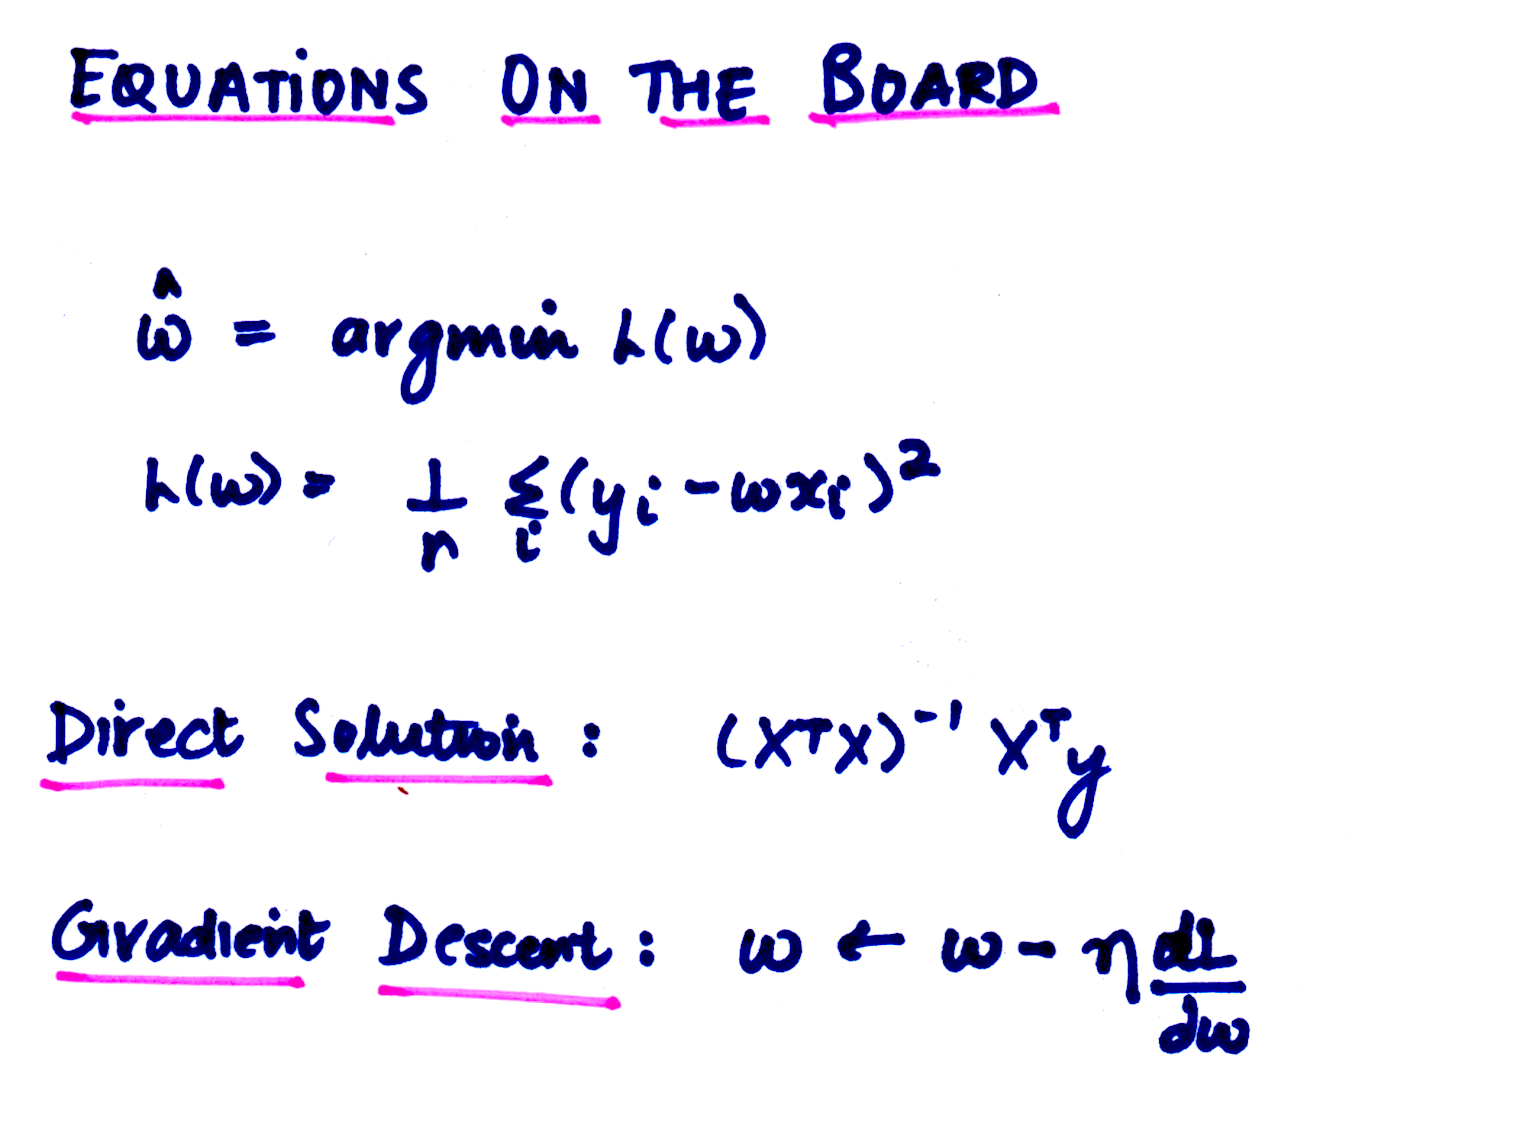
\includegraphics[totalheight=7cm]{1.png}}}
}
\end{figure} 

\section { Model Selection and Evaluation}
The question arises that \emph{When should we stop fitting? }. Here, in the example where we were trying to model internet viewing using age and gender interactions,  we knew that we had to fit a parabola. 
Here we already had the model and we were figuring out how to select the parameters. We did not discuss how to select the model. We usually find the best parameters and visually inspect the fit by plotting the 
predicted and the actual values. 

We summarized the view as average viewing which is not the same as looking at all the ages. If we look at the genders of all the ages in the figure below, we observe that there exists a lot of individual variability 
conditioned on age. The variation between the age is more than the systematic individual variance. The average by age changes a tiny bit. Given that the average changed, doesn't mean every person changed.
This is why it is not such a good model. We can't interpret the model just by staring at the coefficients. There is a lot that has not been explained.  Sometimes, modeling the average is a good idea. If we are making an economic policy, we care about the average more than every individual. Whether we have achieved what we want, depends on the goal. We might want to do analysis \emph {\textbf{quantitatively}} which would actually help us answer if the systematic shift in the mean would explain the variance in the world. Infact, it doesn't and we shall see how simply age and gender does not explain internet viewing!
 
\begin{figure}[h]
\centering
\caption{Internet viewing by gender of all ages}
{\setlength{\fboxsep}{20pt}
\setlength{\fboxrule}{1pt}
\textcolor{Brown}{\fbox {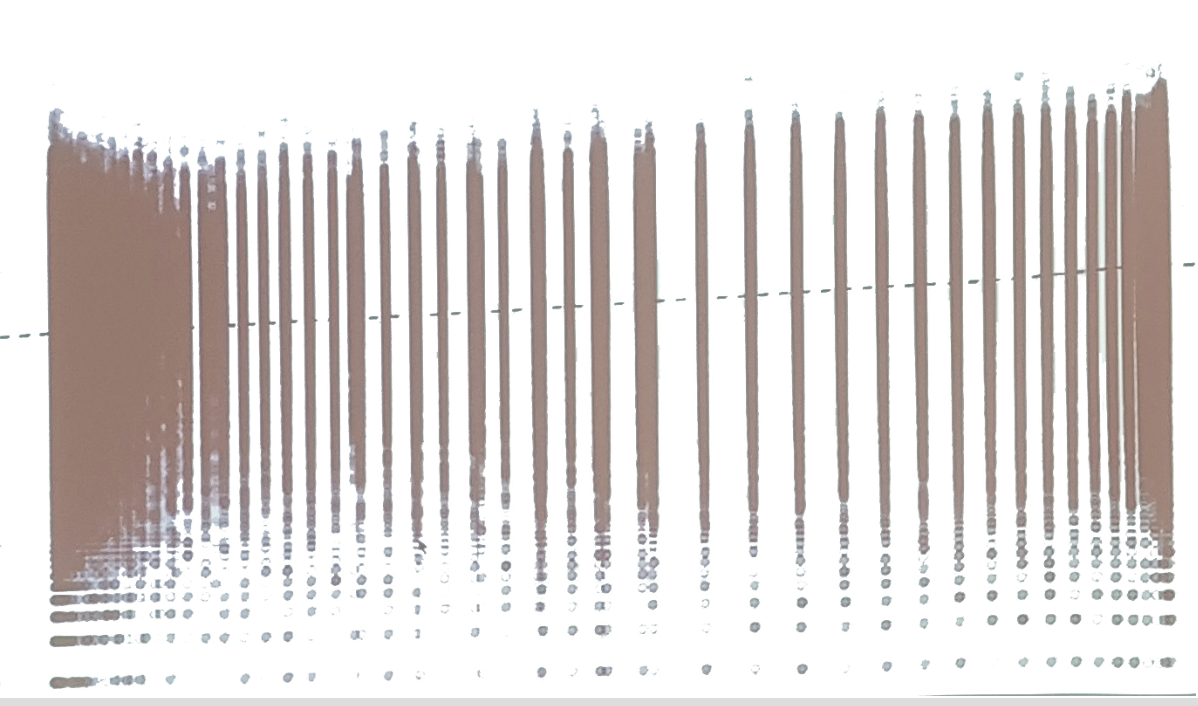
\includegraphics[totalheight=7cm]{var}}}
}
\end{figure} 

\section {Performance metrics for model fitting}
The most common metric for evaluating a model is \emph{Root mean square error.} The square root in the formula is to enforce the same unit. Saying that we are 10000 square page views off doesn't make much sense.
\begin{figure}[h]
\centering
\caption{RMS error}
{\setlength{\fboxsep}{20pt}
\setlength{\fboxrule}{1pt}
\textcolor{DarkBlue}{\fbox {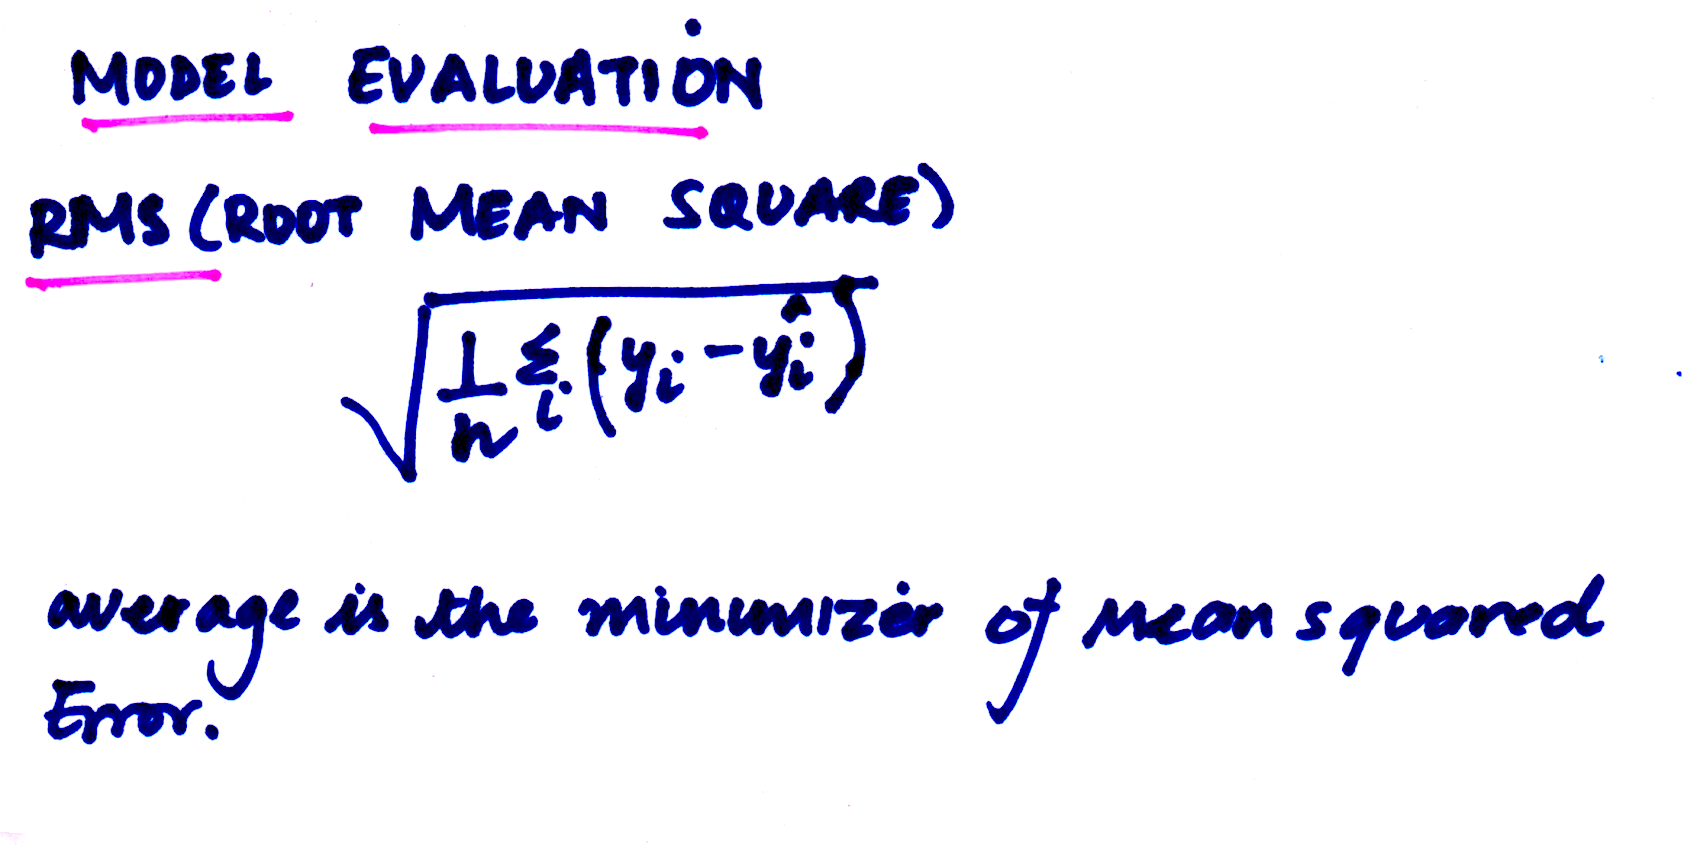
\includegraphics[totalheight=5cm]{2.png}}}
}
\end{figure} 

\newpage
The baseline is to predict the mean for each observation. For any regression problem, we usually measure the performance of the model with respect to the baseline model and ask how does it compare to the average.
The following is the representation of the normalized measure we use to evaluate the model. This measure is called $R^2$.

\begin{figure}[h]
\centering
\caption{$R^2$}
{\setlength{\fboxsep}{20pt}
\setlength{\fboxrule}{1pt}
\textcolor{cyan}{\fbox {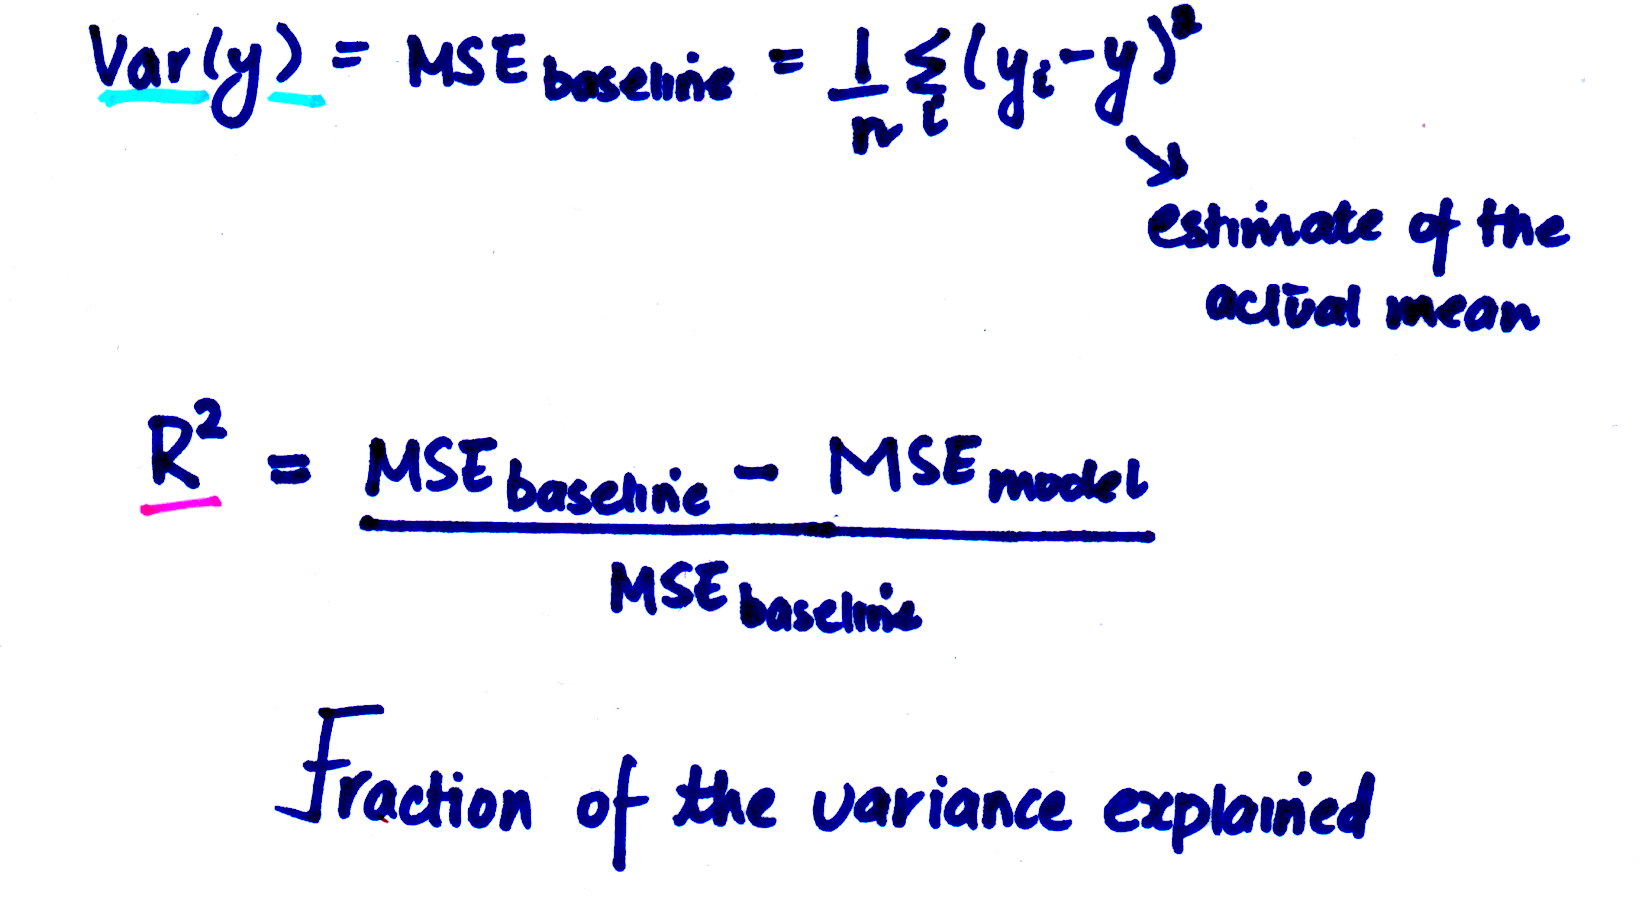
\includegraphics[totalheight=5cm]{4.png}}}
}
\end{figure} 

$R^2$ explains the fraction of variance in the model. The $R$ value of the above model was 0.019 . It means that this model can capture only $2\%$ of the variance of the whole dataset. Terrible! If $R$ is 0, it is pretty bad while if it is 1, the model is great. This value is not unrelated to correlation that is represented by the Pearson's coefficient. The Pearson's coefficient shows how correlated are the deviations of the true and predicted values are, from the mean. We can use features like glance in \emph{R}
to look at the various coefficients. It is very well known that RMS is extremely sensitive to outliers and that big deviations contribute a lot to mean squared error. 

\begin{figure}[h]
\centering
\caption{Pearson's Correlation Coefficient}
{\setlength{\fboxsep}{20pt}
\setlength{\fboxrule}{1pt}
\textcolor{Magenta}{\fbox {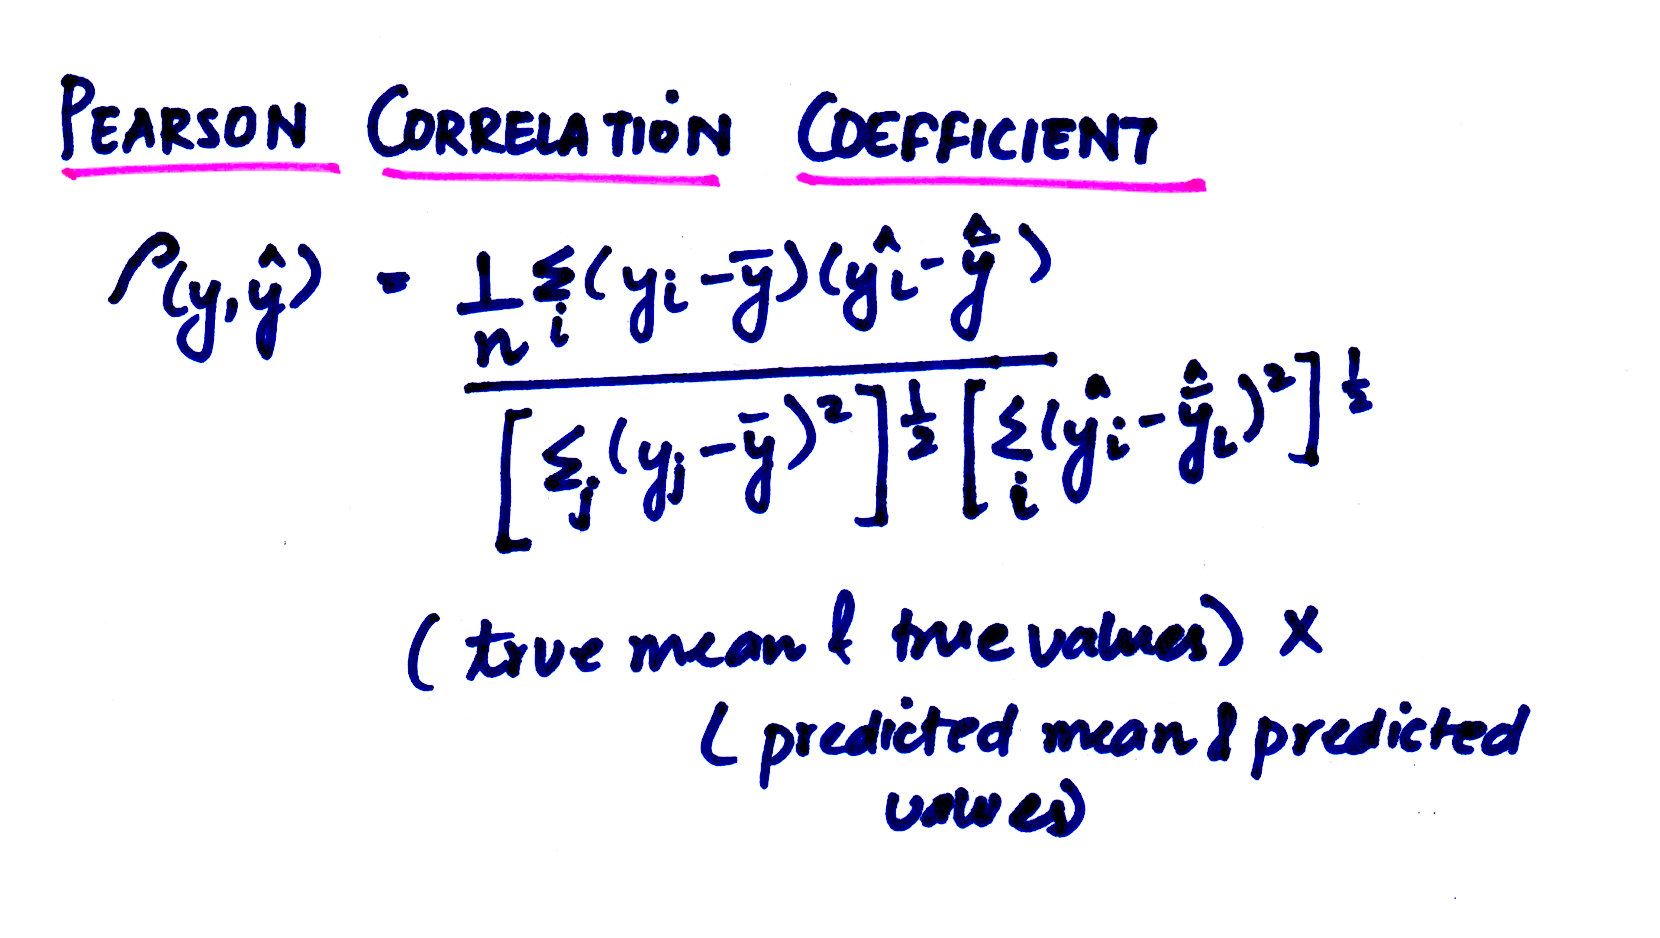
\includegraphics[totalheight=5cm]{3.png}}}
}
\end{figure} 

\newpage
\section{The goal is not to get the training error down to 0!}
While trying to explain the past in your model, you should be careful of not trying to focus on explaining it too well. The goal is to \textbf{generalize} i.e predict well on the unseen data and not try to fit a complex decision boundary that goes through all or most of the training data points. We can use the function $poly(age,k)$ and add more degrees to the decision boundary but this will lead to overfitting. In doing this in \emph{R}, you might get an NA which means that your data points are extremely correlated such that \emph{R} treats them as identical. The thing to remember is that you can do \emph{worse} in the future if pay too much attention to the past.

\subsection {Cross Validation}
The dataset is usually split into three sets - 
\begin{enumerate}
\item Training - This data is used to fit the model and find the best set of parameters. 
\item Test - This should \textbf{not be touched} until we have tested our model on the validation set. 
\item Validation - This data is used to test the performance of the training data before it actually exposed to the test set. We should be careful and should not overfit to the validation set. 
\end{enumerate}
A famous method for validation is \textbf{K-Fold Validation}. Here we select a value of K(generally 5 or 10). A training row is randomly selected and is added to the fold and we go through each fold. 
For each fold, the other K - 1 folds acts as the training data and  the fold selected is treated as the test set. We then select the model with the lowest cross validation error. 

\section{Bias/Variance Tradeoff}

\subsection {Bias?}
Bias is the true error of the best classifier in the concept class (e.g, best linear separator, best decision tree on a fixed number of nodes). Basically, you approximate a function $\hat{f}$ and you compare how much it is off from the true 
function \emph{f}.
\begin{enumerate}
\item High Bias :  If your model has high bias, it means that it assumes something that might not be true, so you could always be off even if you have an infinite amount of training data! 
\item Low Bias : If your model has low bias, it means that it can capture complicated patterns with enough data. For example, if the world is really 9th degree, eventually you will find the right model. 
\end{enumerate}

\subsection {Variance?}
Variance is the error of the trained classifier with respect to the best classifier in the concept class. It is a measure of how much your estimate changes across the different datasets( $\hat{f_1}$,$\hat{f_2}$,$\hat{f_3}$)
\begin{enumerate}
\item High Variance : If your model has high variance, it means your model changes a lot with different training datasets. 
\item Low Variance : If your model has low variance, it means that the estimate doesn't change a lot with different datasets.
\end{enumerate}
\subsection {Tradeoff?}
If we make the concept class more complicated (e.g, linear classification to quadratic classification, or increase number of nodes in the decision tree), then bias decreases but variance increases(Overfitting). On the other hand, if try to lower the variance, we are making the model too simplistic that it cannot capture the true distribution(Underfitting). 
Thus there is a bias-variance tradeoff.

The equation that captures the mean squared error is 
\textbf{MSE $=$ Bias$^2$ + Variance  - Irreducible Error}
 \begin{figure}[h]
\centering
\caption{Generalization Curve}
{\setlength{\fboxsep}{20pt}
\setlength{\fboxrule}{1pt}
\textcolor{cyan}{\fbox {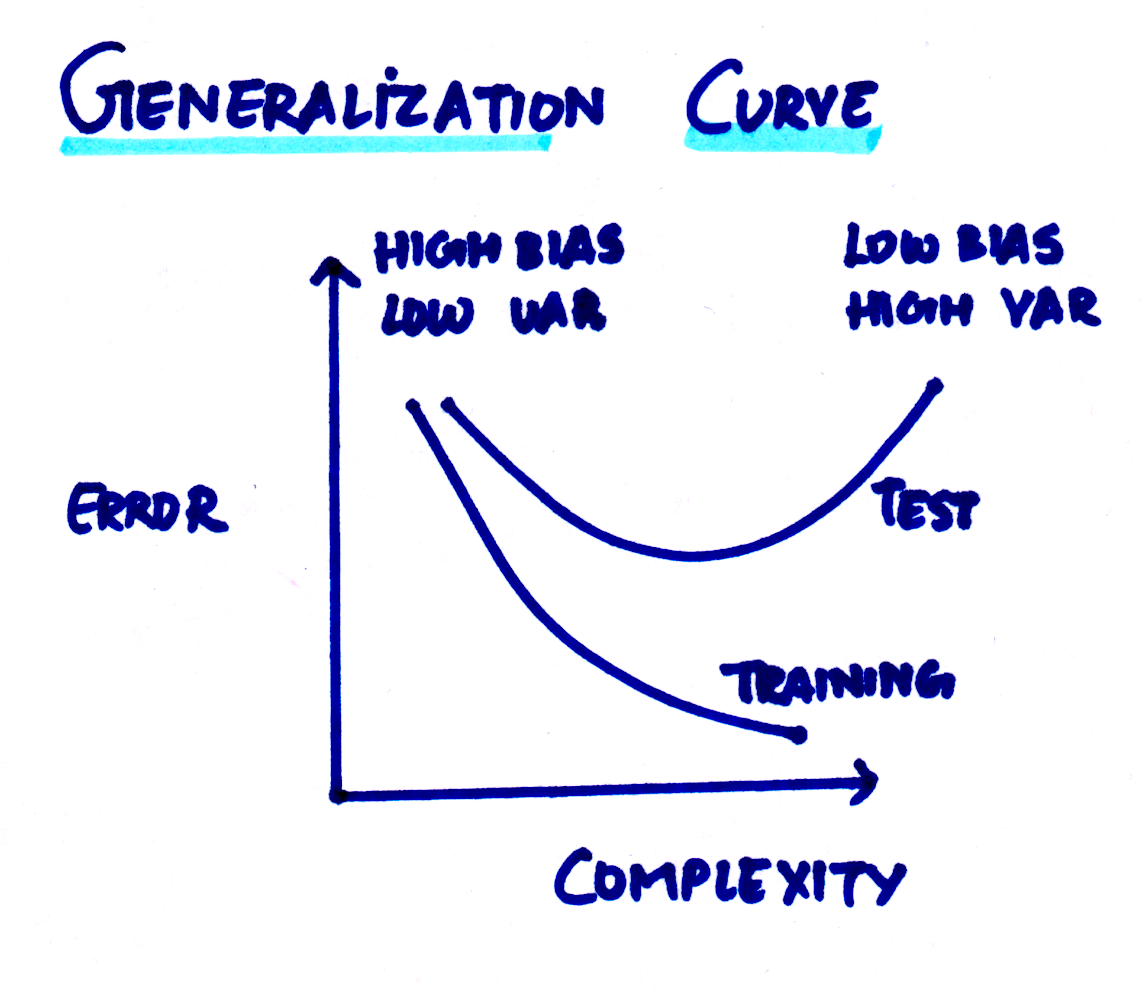
\includegraphics[totalheight=7cm]{5.png}}}
}
\end{figure} 
 
\section{Regularization}
Regularization artificially discourages complex or extreme explanations of the world even if they fit the what has been observed better. The idea is that such explanations are unlikely to generalize well to the future; they may happen to explain a few data points from the past well, but this may just be because of accidents of the sample. It, technically attempts to solve the overfitting problem in statistical models.

\begin{enumerate}
\item{Ridge Regression -  Ridge regression is a way of shrinking weights. It penalizes the loss function using a parameter $\lambda$ times the sum of squared weights. It establishes that it doesn't believe in the weights too much and tries to bring them down in an attempt to generalize well. }
 \begin{figure}[h]
\centering
\caption{Ridge Regression}
{\setlength{\fboxsep}{20pt}
\setlength{\fboxrule}{1pt}
\textcolor{Magenta}{\fbox {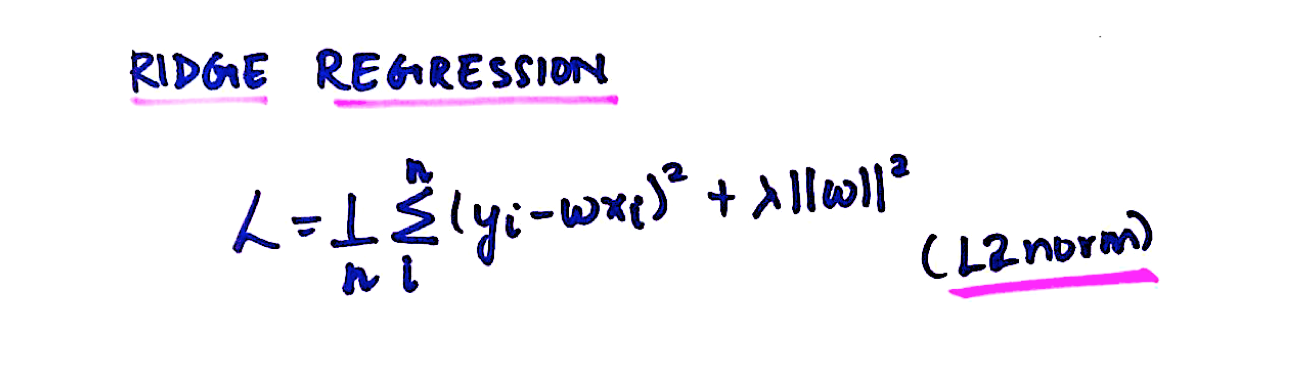
\includegraphics[totalheight=3cm]{ridge.png}}}
}
\end{figure} 
 
\newpage
\item{Lasso Regression -Lasso is a way to perform feature selection. Here, instead of taking the squared norm,we take the absolute norm also known as $L1$ norm. Lasso ropes in a bunch of things and sets them explicitly to zero. It believes that if it had to choose then it would zero out a coefficient than make it small. 
}

 \begin{figure}[h]
\centering
\caption{Lasso Regularization}
{\setlength{\fboxsep}{20pt}
\setlength{\fboxrule}{1pt}
\textcolor{cyan}{\fbox {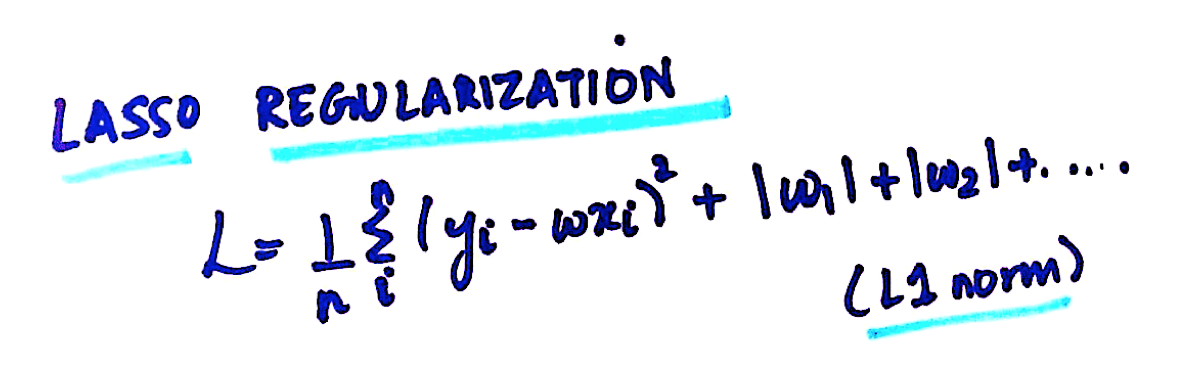
\includegraphics[totalheight=3cm]{las.png}}}
}
\end{figure} 
\end{enumerate}


\section{Bits from the last lecture}
The least squares closed form solution is expensive. It scales in a way such that it would need cubic time ($\mathcal{O}(n^3)$) to perform the operations. 
On huge datasets, cubic times gets really bad. For example, suppose there are 100000 features, we would be processing a 100000 x 100000 matrix.
So, \emph {Gradient Descent} is another option. It should get us to the bottom as the closed form solution. Each one of the steps takes $n*k$ operations. It is computationally
cheap though it has certain downsides. It is iterative and you need to be careful of selecting learning rate $\eta$. For really wide datasets, even $n*k$ operations are a lot. In this case,
we opted for \emph {Stochastic Gradient Descent }. In SGD, we approximate the gradient with a random sample. It helps us control how many points to look at before computing the gradient. 


\begin{figure}[h]
\centering
\caption{Least Square Solutions}
{\setlength{\fboxsep}{20pt}
\setlength{\fboxrule}{1pt}
\textcolor{DarkBlue}{\fbox {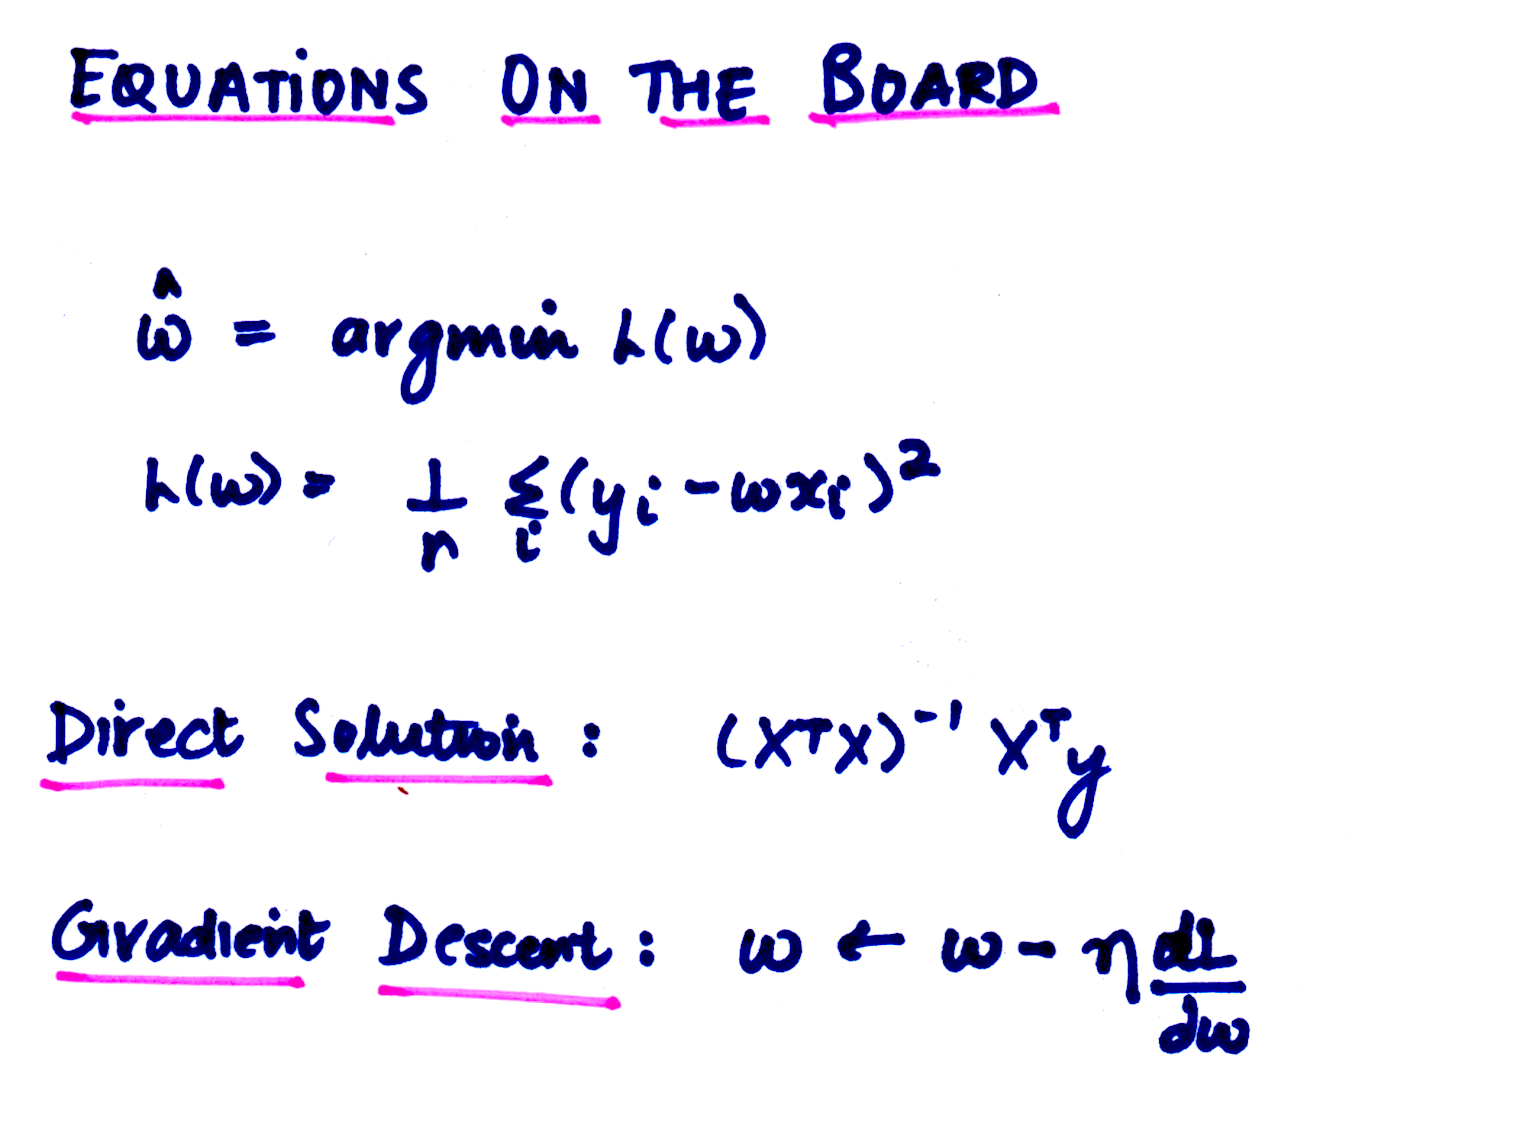
\includegraphics[totalheight=7cm]{1.png}}}
}
\end{figure} 

\section { Model Selection and Evaluation}
The question arises that \emph{When should we stop fitting? }. Here, in the example where we were trying to model internet viewing using age and gender interactions,  we knew that we had to fit a parabola. 
Here we already had the model and we were figuring out how to select the parameters. We did not discuss how to select the model. We usually find the best parameters and visually inspect the fit by plotting the 
predicted and the actual values. 

We summarized the view as average viewing which is not the same as looking at all the ages. If we look at the genders of all the ages in the figure below, we observe that there exists a lot of individual variability 
conditioned on age. The variation between the age is more than the systematic individual variance. The average by age changes a tiny bit. Given that the average changed, doesn't mean every person changed.
This is why it is not such a good model. We can't interpret the model just by staring at the coefficients. There is a lot that has not been explained.  Sometimes, modeling the average is a good idea. If we are making an economic policy, we care about the average more than every individual. Whether we have achieved what we want, depends on the goal. We might want to do analysis \emph {\textbf{quantitatively}} which would actually help us answer if the systematic shift in the mean would explain the variance in the world. Infact, it doesn't and we shall see how simply age and gender does not explain internet viewing!
 
\begin{figure}[h]
\centering
\caption{Internet viewing by gender of all ages}
{\setlength{\fboxsep}{20pt}
\setlength{\fboxrule}{1pt}
\textcolor{Brown}{\fbox {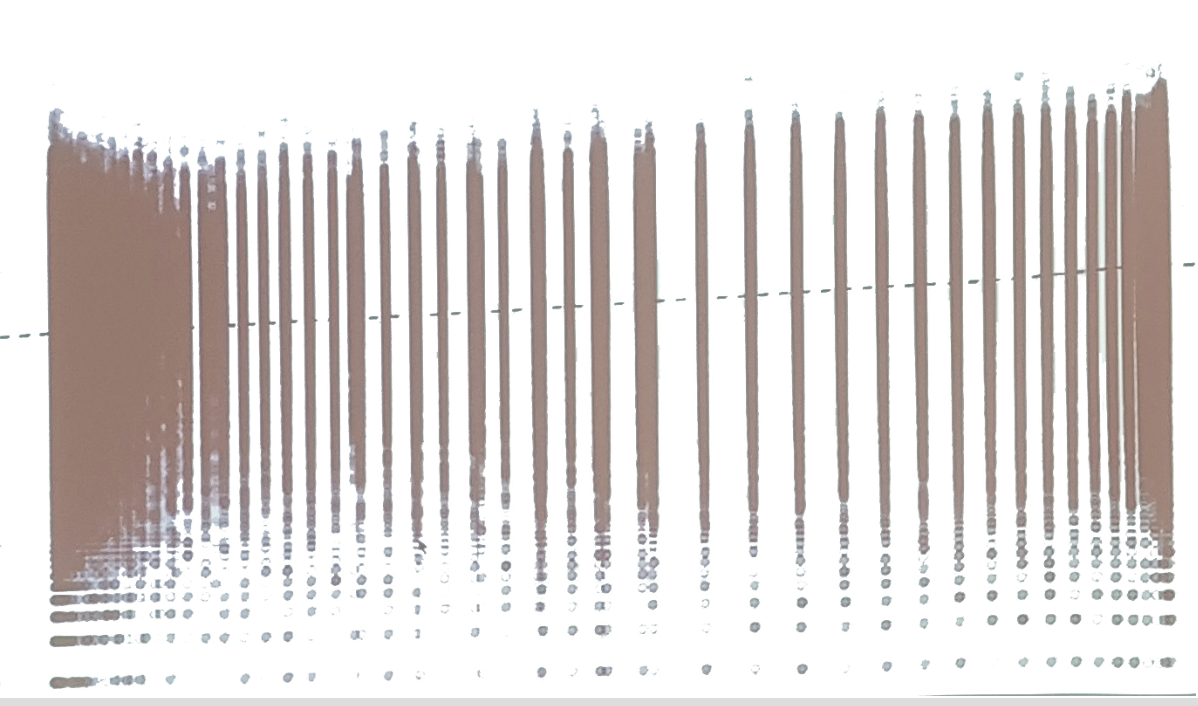
\includegraphics[totalheight=7cm]{var}}}
}
\end{figure} 

\section {Performance metrics for model fitting}
The most common metric for evaluating a model is \emph{Root mean square error.} The square root in the formula is to enforce the same unit. Saying that we are 10000 square page views off doesn't make much sense.
\begin{figure}[h]
\centering
\caption{RMS error}
{\setlength{\fboxsep}{20pt}
\setlength{\fboxrule}{1pt}
\textcolor{DarkBlue}{\fbox {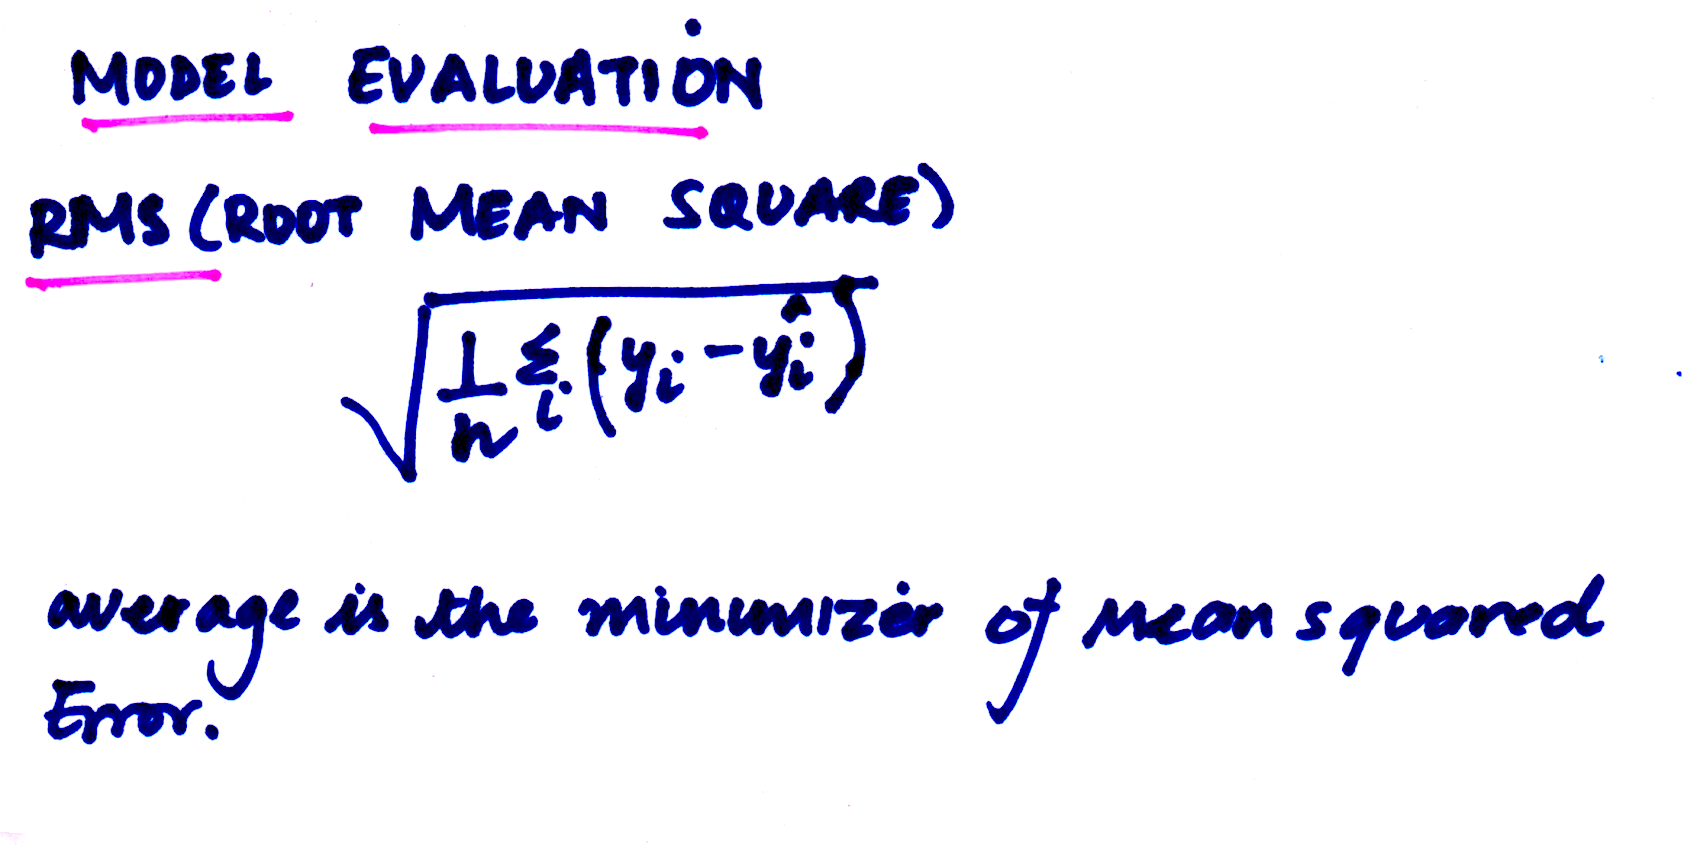
\includegraphics[totalheight=5cm]{2.png}}}
}
\end{figure} 

\newpage
The baseline is to predict the mean for each observation. For any regression problem, we usually measure the performance of the model with respect to the baseline model and ask how does it compare to the average.
The following is the representation of the normalized measure we use to evaluate the model. This measure is called $R^2$.

\begin{figure}[h]
\centering
\caption{$R^2$}
{\setlength{\fboxsep}{20pt}
\setlength{\fboxrule}{1pt}
\textcolor{cyan}{\fbox {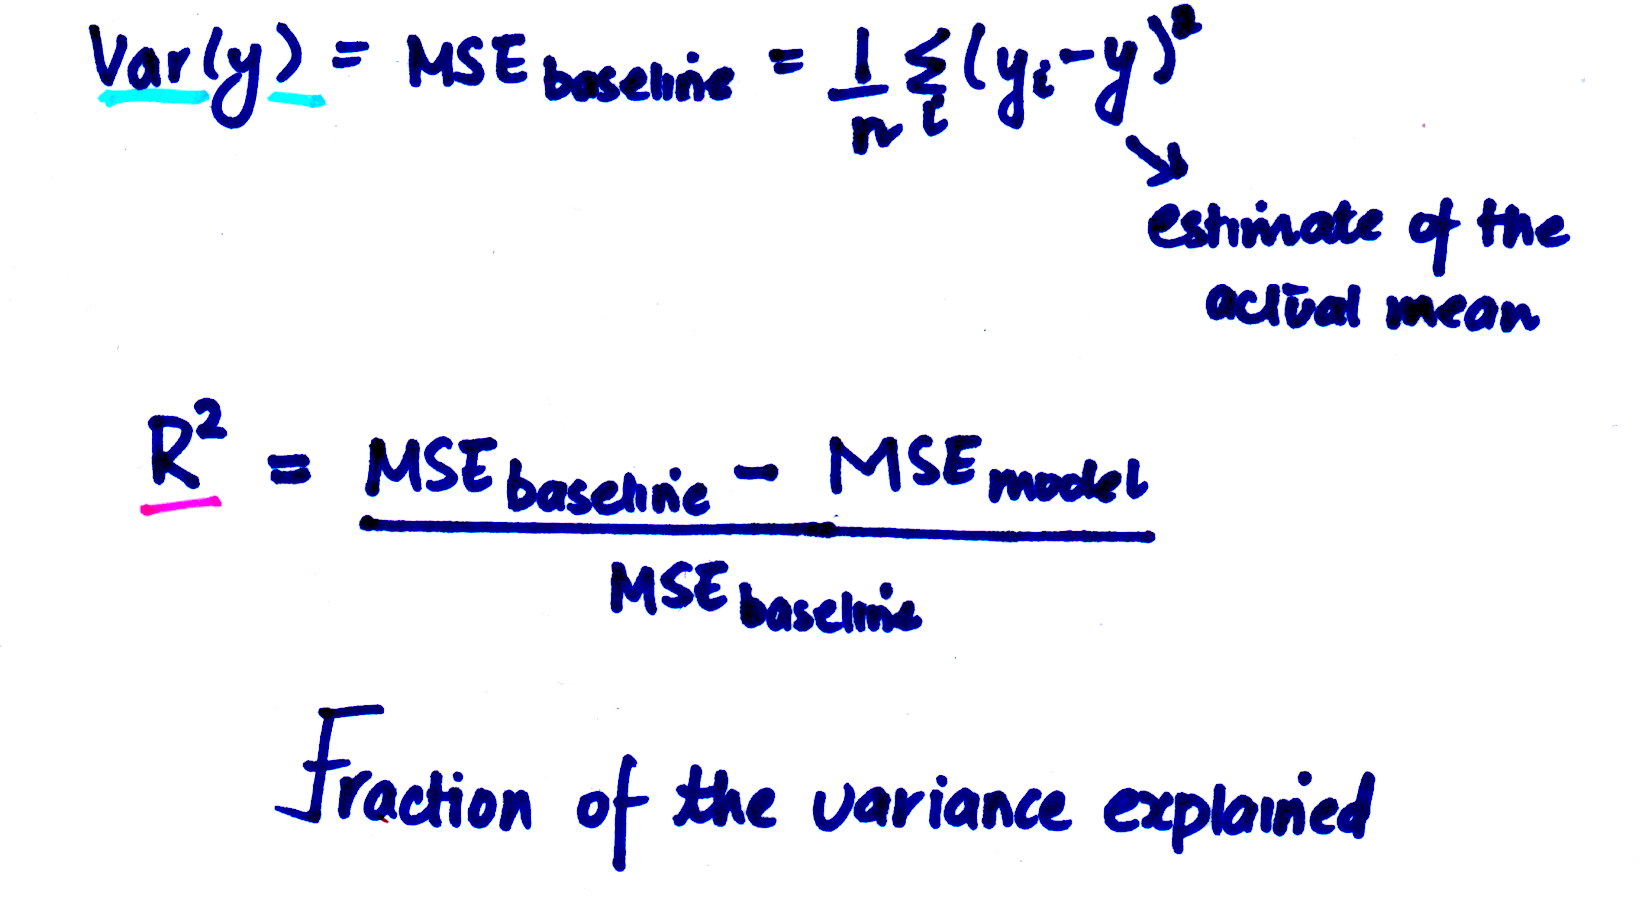
\includegraphics[totalheight=5cm]{4.png}}}
}
\end{figure} 

$R^2$ explains the fraction of variance in the model. The $R$ value of the above model was 0.019 . It means that this model can capture only $2\%$ of the variance of the whole dataset. Terrible! If $R$ is 0, it is pretty bad while if it is 1, the model is great. This value is not unrelated to correlation that is represented by the Pearson's coefficient. The Pearson's coefficient shows how correlated are the deviations of the true and predicted values are, from the mean. We can use features like glance in \emph{R}
to look at the various coefficients. It is very well known that RMS is extremely sensitive to outliers and that big deviations contribute a lot to mean squared error. 

\begin{figure}[h]
\centering
\caption{Pearson's Correlation Coefficient}
{\setlength{\fboxsep}{20pt}
\setlength{\fboxrule}{1pt}
\textcolor{Magenta}{\fbox {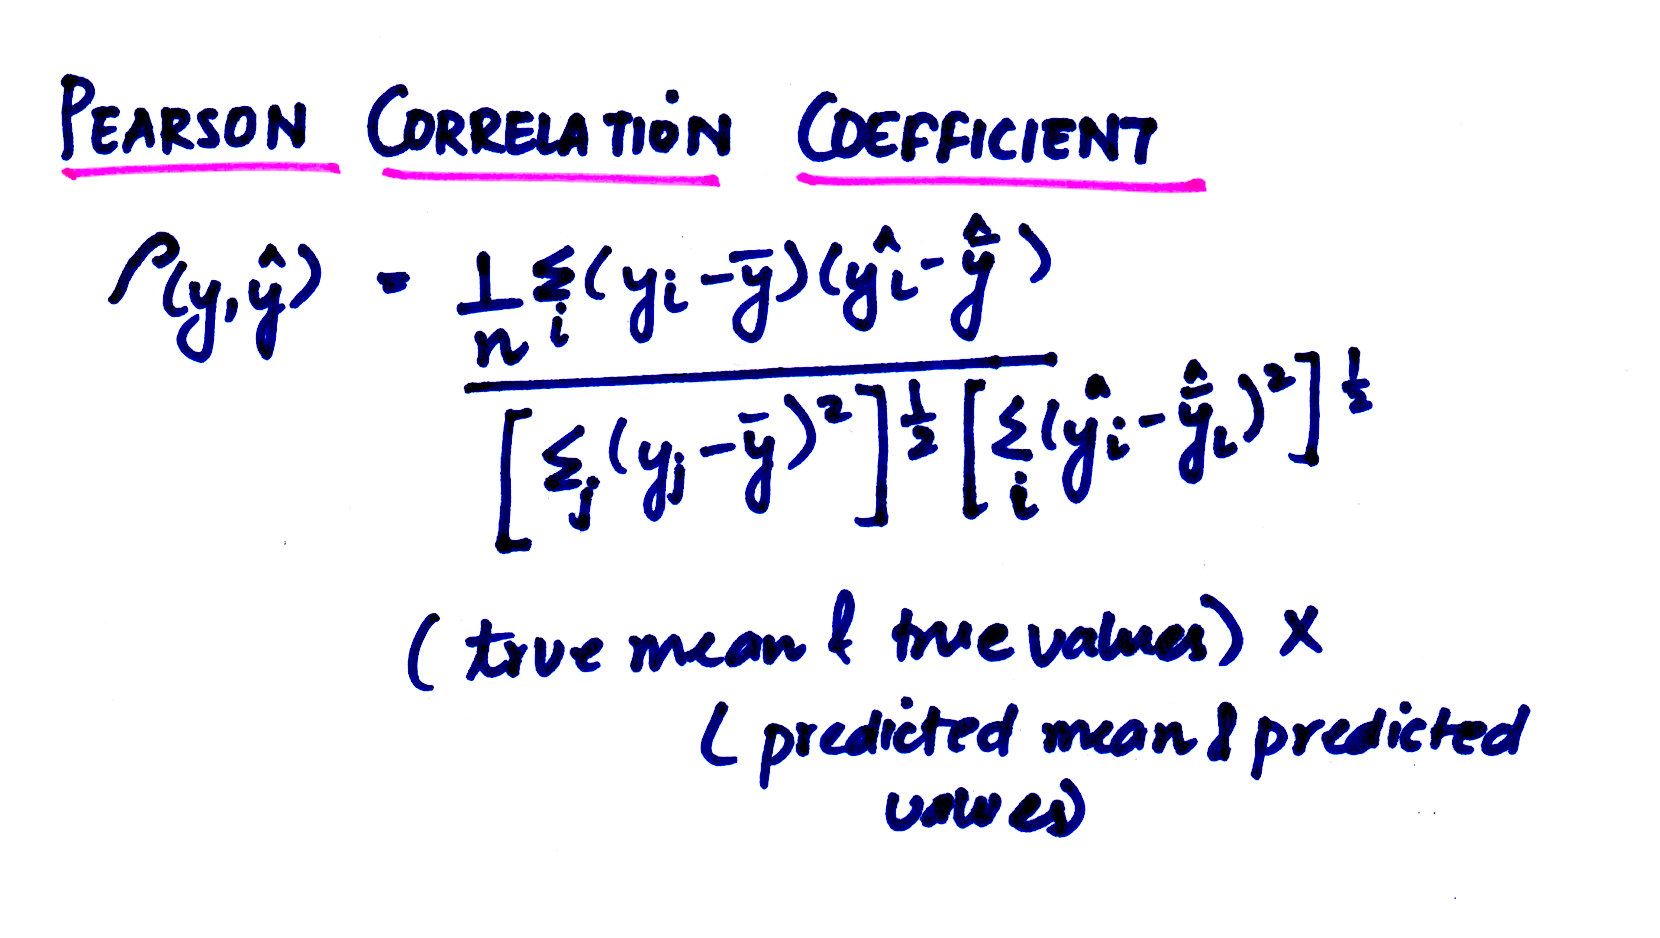
\includegraphics[totalheight=5cm]{3.png}}}
}
\end{figure} 

\newpage
\section{The goal is not to get the training error down to 0!}
While trying to explain the past in your model, you should be careful of not trying to focus on explaining it too well. The goal is to \textbf{generalize} i.e predict well on the unseen data and not try to fit a complex decision boundary that goes through all or most of the training data points. We can use the function $poly(age,k)$ and add more degrees to the decision boundary but this will lead to overfitting. In doing this in \emph{R}, you might get an NA which means that your data points are extremely correlated such that \emph{R} treats them as identical. The thing to remember is that you can do \emph{worse} in the future if pay too much attention to the past.

\subsection {Cross Validation}
The dataset is usually split into three sets - 
\begin{enumerate}
\item Training - This data is used to fit the model and find the best set of parameters. 
\item Test - This should \textbf{not be touched} until we have tested our model on the validation set. 
\item Validation - This data is used to test the performance of the training data before it actually exposed to the test set. We should be careful and should not overfit to the validation set. 
\end{enumerate}
A famous method for validation is \textbf{K-Fold Validation}. Here we select a value of K(generally 5 or 10). A training row is randomly selected and is added to the fold and we go through each fold. 
For each fold, the other K - 1 folds acts as the training data and  the fold selected is treated as the test set. We then select the model with the lowest cross validation error. 

\section{Bias/Variance Tradeoff}

\subsection {Bias?}
Bias is the true error of the best classifier in the concept class (e.g, best linear separator, best decision tree on a fixed number of nodes). Basically, you approximate a function $\hat{f}$ and you compare how much it is off from the true 
function \emph{f}.
\begin{enumerate}
\item High Bias :  If your model has high bias, it means that it assumes something that might not be true, so you could always be off even if you have an infinite amount of training data! 
\item Low Bias : If your model has low bias, it means that it can capture complicated patterns with enough data. For example, if the world is really 9th degree, eventually you will find the right model. 
\end{enumerate}

\subsection {Variance?}
Variance is the error of the trained classifier with respect to the best classifier in the concept class. It is a measure of how much your estimate changes across the different datasets( $\hat{f_1}$,$\hat{f_2}$,$\hat{f_3}$)
\begin{enumerate}
\item High Variance : If your model has high variance, it means your model changes a lot with different training datasets. 
\item Low Variance : If your model has low variance, it means that the estimate doesn't change a lot with different datasets.
\end{enumerate}
\subsection {Tradeoff?}
If we make the concept class more complicated (e.g, linear classification to quadratic classification, or increase number of nodes in the decision tree), then bias decreases but variance increases(Overfitting). On the other hand, if try to lower the variance, we are making the model too simplistic that it cannot capture the true distribution(Underfitting). 
Thus there is a bias-variance tradeoff.

The equation that captures the mean squared error is 
\textbf{MSE $=$ Bias$^2$ + Variance  - Irreducible Error}
 \begin{figure}[h]
\centering
\caption{Generalization Curve}
{\setlength{\fboxsep}{20pt}
\setlength{\fboxrule}{1pt}
\textcolor{cyan}{\fbox {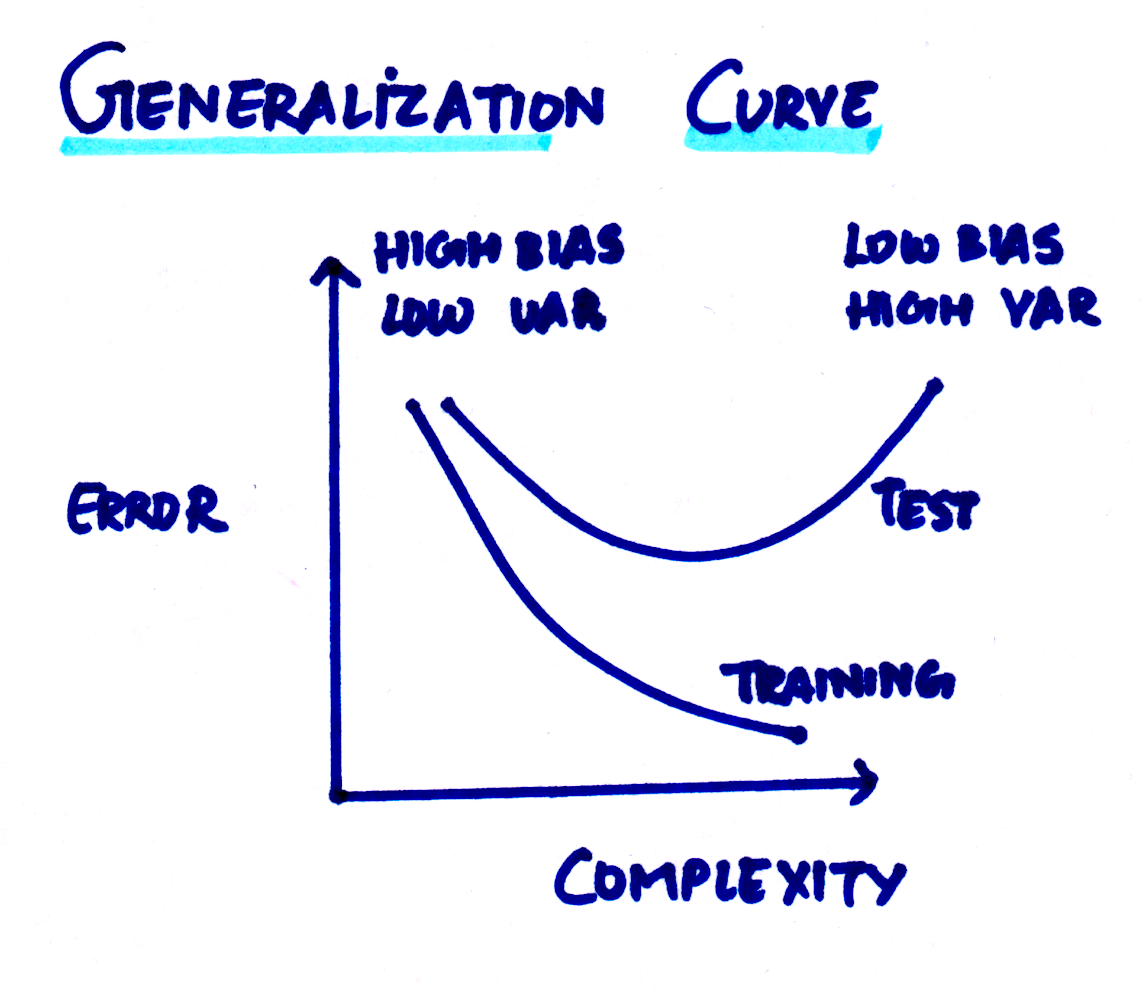
\includegraphics[totalheight=7cm]{5.png}}}
}
\end{figure} 
 
\section{Regularization}
Regularization artificially discourages complex or extreme explanations of the world even if they fit the what has been observed better. The idea is that such explanations are unlikely to generalize well to the future; they may happen to explain a few data points from the past well, but this may just be because of accidents of the sample. It, technically attempts to solve the overfitting problem in statistical models.

\begin{enumerate}
\item{Ridge Regression -  Ridge regression is a way of shrinking weights. It penalizes the loss function using a parameter $\lambda$ times the sum of squared weights. It establishes that it doesn't believe in the weights too much and tries to bring them down in an attempt to generalize well. }
 \begin{figure}[h]
\centering
\caption{Ridge Regression}
{\setlength{\fboxsep}{20pt}
\setlength{\fboxrule}{1pt}
\textcolor{Magenta}{\fbox {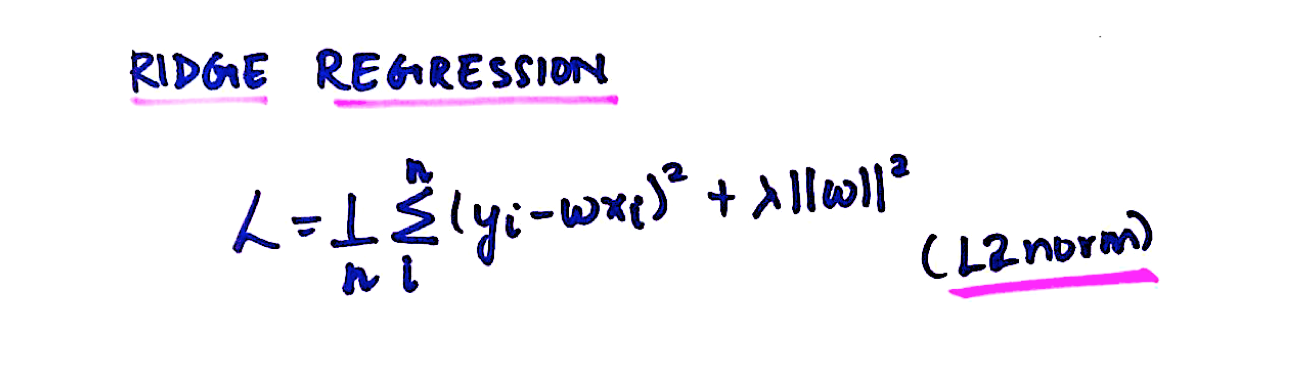
\includegraphics[totalheight=3cm]{ridge.png}}}
}
\end{figure} 
 
\newpage
\item{Lasso Regression -Lasso is a way to perform feature selection. Here, instead of taking the squared norm,we take the absolute norm also known as $L1$ norm. Lasso ropes in a bunch of things and sets them explicitly to zero. It believes that if it had to choose then it would zero out a coefficient than make it small. 
}

 \begin{figure}[h]
\centering
\caption{Lasso Regularization}
{\setlength{\fboxsep}{20pt}
\setlength{\fboxrule}{1pt}
\textcolor{cyan}{\fbox {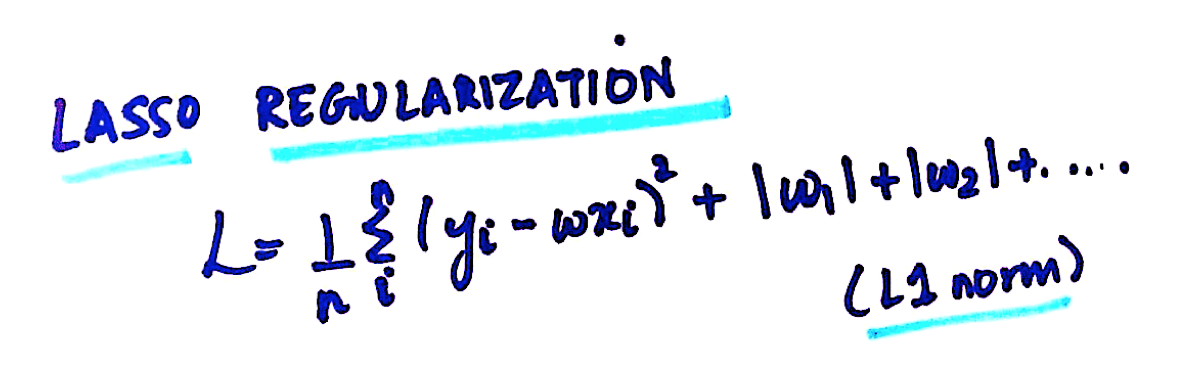
\includegraphics[totalheight=3cm]{las.png}}}
}
\end{figure} 
\end{enumerate}


\end{document}

%%% Local Variables:
%%% mode: latex
%%% TeX-master: t
%%% End: